\documentclass[12pt]{article}
\usepackage[letterpaper, left=0.75in, right=0.75in, top=0.85in, bottom=0.85in, headsep=0.25in, footskip=0.4in]{geometry}
\usepackage[T1]{fontenc}
\usepackage[scaled=0.95]{helvet}
\renewcommand{\familydefault}{\sfdefault}
\usepackage{tikz}
\usetikzlibrary{arrows.meta}
\usepackage{fancyhdr}
\pagestyle{fancy}
\fancyhf{}
\renewcommand{\headrulewidth}{0pt}
\lhead{\small Week NN / Pancake flips / Grades 2--3}
\lfoot{\small Bellingham Math Circle / Week NN / NN-23-v1}
\rfoot{\small \thepage}
\setlength{\parindent}{0pt}
\setlength{\parskip}{6pt}
\definecolor{cakefillc}{RGB}{248,224,170}
\definecolor{cakedrawc}{RGB}{140,95,35}
\definecolor{burntc}{RGB}{85,50,20}
\tikzset{
  cakefill/.style={fill=cakefillc},
  cakedraw/.style={draw=cakedrawc, line width=0.9pt},
  burnt/.style={fill=burntc},
  platedraw/.style={draw=black!55, line width=0.6pt},
  platefill/.style={fill=black!18},
  slot/.style={draw=black!70, dashed, line width=0.8pt},
  spatula/.style={fill=black!65},
  handle/.style={fill=black!40},
  tokdraw/.style={draw=black!70, line width=0.8pt},
  tokfill/.style={fill=black!12},
  breakmark/.style={draw=red!80!black, line width=1.8pt, line cap=round},
}
\newcommand{\problem}[1]{\par\medskip\textbf{Problem #1:}\ }
\begin{document}
A stack is sorted when each pancake sits on a bigger one. To flip, slide the spatula under any pancake and turn that pancake and everything above it over together. Write a stack as its numbers from the top, and a flip as the number of pancakes it turns over.
\par\smallskip\begin{center}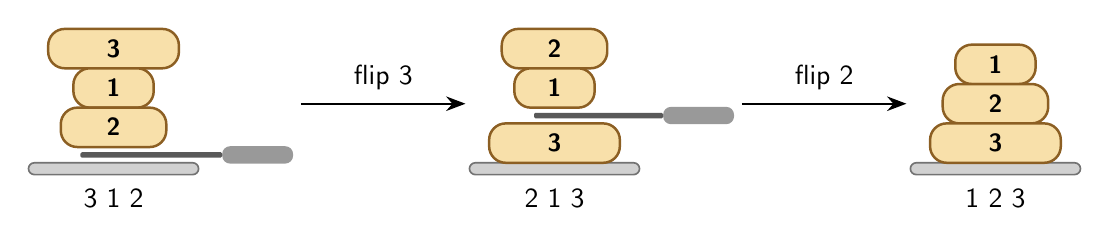
\begin{tikzpicture}
\draw[platedraw, platefill, rounded corners=0.075cm] (-1.080,-0.150) rectangle (1.080,0);
\fill[cakefill] [rounded corners=0.210cm] (-0.830,1.200) rectangle (0.830,1.700);
\draw[cakedraw] [rounded corners=0.210cm] (-0.830,1.200) rectangle (0.830,1.700);
\node[font=\small\bfseries, inner sep=0pt] at (0.000,1.450) {3};
\fill[cakefill] [rounded corners=0.210cm] (-0.510,0.700) rectangle (0.510,1.200);
\draw[cakedraw] [rounded corners=0.210cm] (-0.510,0.700) rectangle (0.510,1.200);
\node[font=\small\bfseries, inner sep=0pt] at (0.000,0.950) {1};
\fill[cakefill] [rounded corners=0.210cm] (-0.670,0.200) rectangle (0.670,0.700);
\draw[cakedraw] [rounded corners=0.210cm] (-0.670,0.200) rectangle (0.670,0.700);
\node[font=\small\bfseries, inner sep=0pt] at (0.000,0.450) {2};
\fill[spatula, rounded corners=0.5pt] (-0.420,0.065) rectangle (1.380,0.135);
\fill[handle, rounded corners=0.099cm] (1.380,-0.010) rectangle (2.280,0.210);
\node[anchor=north, font=\normalsize, inner sep=0pt] at (0.000,-0.330) {3\,\,1\,\,2};
\draw[-{Stealth[length=7pt]}, thick] (2.380,0.750) -- (4.470,0.750);
\node[above, font=\normalsize] at (3.425,0.800) {flip 3};
\draw[platedraw, platefill, rounded corners=0.075cm] (4.520,-0.150) rectangle (6.680,0);
\fill[cakefill] [rounded corners=0.210cm] (4.930,1.200) rectangle (6.270,1.700);
\draw[cakedraw] [rounded corners=0.210cm] (4.930,1.200) rectangle (6.270,1.700);
\node[font=\small\bfseries, inner sep=0pt] at (5.600,1.450) {2};
\fill[cakefill] [rounded corners=0.210cm] (5.090,0.700) rectangle (6.110,1.200);
\draw[cakedraw] [rounded corners=0.210cm] (5.090,0.700) rectangle (6.110,1.200);
\node[font=\small\bfseries, inner sep=0pt] at (5.600,0.950) {1};
\fill[cakefill] [rounded corners=0.210cm] (4.770,0.000) rectangle (6.430,0.500);
\draw[cakedraw] [rounded corners=0.210cm] (4.770,0.000) rectangle (6.430,0.500);
\node[font=\small\bfseries, inner sep=0pt] at (5.600,0.250) {3};
\fill[spatula, rounded corners=0.5pt] (5.340,0.565) rectangle (6.980,0.635);
\fill[handle, rounded corners=0.099cm] (6.980,0.490) rectangle (7.880,0.710);
\node[anchor=north, font=\normalsize, inner sep=0pt] at (5.600,-0.330) {2\,\,1\,\,3};
\draw[-{Stealth[length=7pt]}, thick] (7.980,0.750) -- (10.070,0.750);
\node[above, font=\normalsize] at (9.025,0.800) {flip 2};
\draw[platedraw, platefill, rounded corners=0.075cm] (10.120,-0.150) rectangle (12.280,0);
\fill[cakefill] [rounded corners=0.210cm] (10.690,1.000) rectangle (11.710,1.500);
\draw[cakedraw] [rounded corners=0.210cm] (10.690,1.000) rectangle (11.710,1.500);
\node[font=\small\bfseries, inner sep=0pt] at (11.200,1.250) {1};
\fill[cakefill] [rounded corners=0.210cm] (10.530,0.500) rectangle (11.870,1.000);
\draw[cakedraw] [rounded corners=0.210cm] (10.530,0.500) rectangle (11.870,1.000);
\node[font=\small\bfseries, inner sep=0pt] at (11.200,0.750) {2};
\fill[cakefill] [rounded corners=0.210cm] (10.370,0.000) rectangle (12.030,0.500);
\draw[cakedraw] [rounded corners=0.210cm] (10.370,0.000) rectangle (12.030,0.500);
\node[font=\small\bfseries, inner sep=0pt] at (11.200,0.250) {3};
\node[anchor=north, font=\normalsize, inner sep=0pt] at (11.200,-0.330) {1\,\,2\,\,3};
\end{tikzpicture}\end{center}
\problem{1}Sort each stack with as few flips as you can. Write down your flips.
\par\medskip
\noindent\makebox[\linewidth][s]{\hfill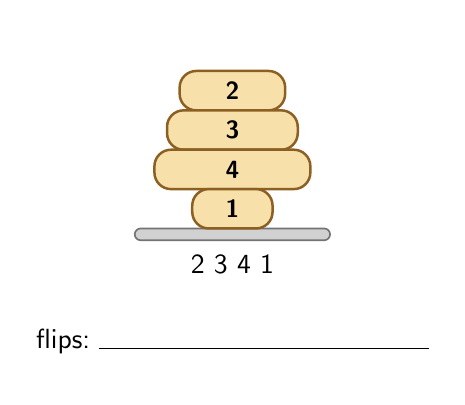
\begin{tikzpicture}
\useasboundingbox (-2.600,-1.880) rectangle (2.600,2.550);
\draw[platedraw, platefill, rounded corners=0.075cm] (-1.240,-0.150) rectangle (1.240,0);
\fill[cakefill] [rounded corners=0.210cm] (-0.670,1.500) rectangle (0.670,2.000);
\draw[cakedraw] [rounded corners=0.210cm] (-0.670,1.500) rectangle (0.670,2.000);
\node[font=\small\bfseries, inner sep=0pt] at (0.000,1.750) {2};
\fill[cakefill] [rounded corners=0.210cm] (-0.830,1.000) rectangle (0.830,1.500);
\draw[cakedraw] [rounded corners=0.210cm] (-0.830,1.000) rectangle (0.830,1.500);
\node[font=\small\bfseries, inner sep=0pt] at (0.000,1.250) {3};
\fill[cakefill] [rounded corners=0.210cm] (-0.990,0.500) rectangle (0.990,1.000);
\draw[cakedraw] [rounded corners=0.210cm] (-0.990,0.500) rectangle (0.990,1.000);
\node[font=\small\bfseries, inner sep=0pt] at (0.000,0.750) {4};
\fill[cakefill] [rounded corners=0.210cm] (-0.510,0.000) rectangle (0.510,0.500);
\draw[cakedraw] [rounded corners=0.210cm] (-0.510,0.000) rectangle (0.510,0.500);
\node[font=\small\bfseries, inner sep=0pt] at (0.000,0.250) {1};
\node[anchor=north, font=\normalsize, inner sep=0pt] at (0.000,-0.330) {2\,\,3\,\,4\,\,1};
\node[anchor=base west, font=\normalsize, inner sep=0pt] (fl) at (-2.500,-1.530) {flips:};
\draw[thin] ([xshift=3pt]fl.base east) -- (2.500,-1.530);
\end{tikzpicture}\hfill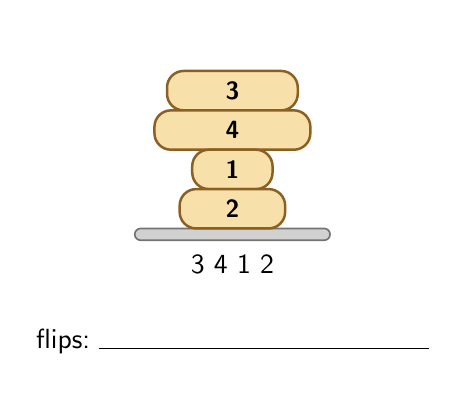
\begin{tikzpicture}
\useasboundingbox (-2.600,-1.880) rectangle (2.600,2.550);
\draw[platedraw, platefill, rounded corners=0.075cm] (-1.240,-0.150) rectangle (1.240,0);
\fill[cakefill] [rounded corners=0.210cm] (-0.830,1.500) rectangle (0.830,2.000);
\draw[cakedraw] [rounded corners=0.210cm] (-0.830,1.500) rectangle (0.830,2.000);
\node[font=\small\bfseries, inner sep=0pt] at (0.000,1.750) {3};
\fill[cakefill] [rounded corners=0.210cm] (-0.990,1.000) rectangle (0.990,1.500);
\draw[cakedraw] [rounded corners=0.210cm] (-0.990,1.000) rectangle (0.990,1.500);
\node[font=\small\bfseries, inner sep=0pt] at (0.000,1.250) {4};
\fill[cakefill] [rounded corners=0.210cm] (-0.510,0.500) rectangle (0.510,1.000);
\draw[cakedraw] [rounded corners=0.210cm] (-0.510,0.500) rectangle (0.510,1.000);
\node[font=\small\bfseries, inner sep=0pt] at (0.000,0.750) {1};
\fill[cakefill] [rounded corners=0.210cm] (-0.670,0.000) rectangle (0.670,0.500);
\draw[cakedraw] [rounded corners=0.210cm] (-0.670,0.000) rectangle (0.670,0.500);
\node[font=\small\bfseries, inner sep=0pt] at (0.000,0.250) {2};
\node[anchor=north, font=\normalsize, inner sep=0pt] at (0.000,-0.330) {3\,\,4\,\,1\,\,2};
\node[anchor=base west, font=\normalsize, inner sep=0pt] (fl) at (-2.500,-1.530) {flips:};
\draw[thin] ([xshift=3pt]fl.base east) -- (2.500,-1.530);
\end{tikzpicture}\hfill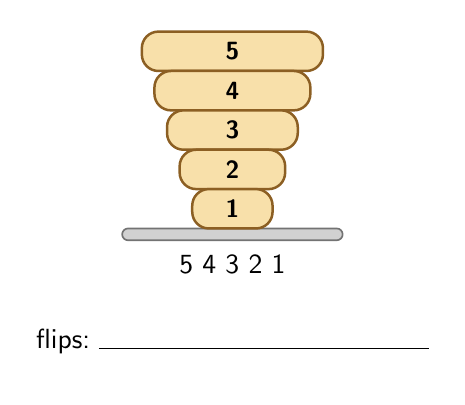
\begin{tikzpicture}
\useasboundingbox (-2.600,-1.880) rectangle (2.600,2.550);
\draw[platedraw, platefill, rounded corners=0.075cm] (-1.400,-0.150) rectangle (1.400,0);
\fill[cakefill] [rounded corners=0.210cm] (-1.150,2.000) rectangle (1.150,2.500);
\draw[cakedraw] [rounded corners=0.210cm] (-1.150,2.000) rectangle (1.150,2.500);
\node[font=\small\bfseries, inner sep=0pt] at (0.000,2.250) {5};
\fill[cakefill] [rounded corners=0.210cm] (-0.990,1.500) rectangle (0.990,2.000);
\draw[cakedraw] [rounded corners=0.210cm] (-0.990,1.500) rectangle (0.990,2.000);
\node[font=\small\bfseries, inner sep=0pt] at (0.000,1.750) {4};
\fill[cakefill] [rounded corners=0.210cm] (-0.830,1.000) rectangle (0.830,1.500);
\draw[cakedraw] [rounded corners=0.210cm] (-0.830,1.000) rectangle (0.830,1.500);
\node[font=\small\bfseries, inner sep=0pt] at (0.000,1.250) {3};
\fill[cakefill] [rounded corners=0.210cm] (-0.670,0.500) rectangle (0.670,1.000);
\draw[cakedraw] [rounded corners=0.210cm] (-0.670,0.500) rectangle (0.670,1.000);
\node[font=\small\bfseries, inner sep=0pt] at (0.000,0.750) {2};
\fill[cakefill] [rounded corners=0.210cm] (-0.510,0.000) rectangle (0.510,0.500);
\draw[cakedraw] [rounded corners=0.210cm] (-0.510,0.000) rectangle (0.510,0.500);
\node[font=\small\bfseries, inner sep=0pt] at (0.000,0.250) {1};
\node[anchor=north, font=\normalsize, inner sep=0pt] at (0.000,-0.330) {5\,\,4\,\,3\,\,2\,\,1};
\node[anchor=base west, font=\normalsize, inner sep=0pt] (fl) at (-2.500,-1.530) {flips:};
\draw[thin] ([xshift=3pt]fl.base east) -- (2.500,-1.530);
\end{tikzpicture}\hfill}

\par\vspace{0.6cm}
\noindent\makebox[\linewidth][s]{\hfill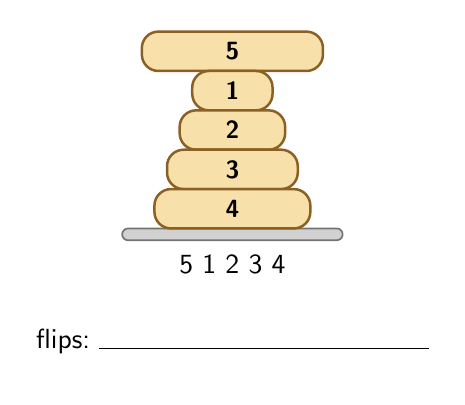
\begin{tikzpicture}
\useasboundingbox (-2.600,-1.880) rectangle (2.600,2.550);
\draw[platedraw, platefill, rounded corners=0.075cm] (-1.400,-0.150) rectangle (1.400,0);
\fill[cakefill] [rounded corners=0.210cm] (-1.150,2.000) rectangle (1.150,2.500);
\draw[cakedraw] [rounded corners=0.210cm] (-1.150,2.000) rectangle (1.150,2.500);
\node[font=\small\bfseries, inner sep=0pt] at (0.000,2.250) {5};
\fill[cakefill] [rounded corners=0.210cm] (-0.510,1.500) rectangle (0.510,2.000);
\draw[cakedraw] [rounded corners=0.210cm] (-0.510,1.500) rectangle (0.510,2.000);
\node[font=\small\bfseries, inner sep=0pt] at (0.000,1.750) {1};
\fill[cakefill] [rounded corners=0.210cm] (-0.670,1.000) rectangle (0.670,1.500);
\draw[cakedraw] [rounded corners=0.210cm] (-0.670,1.000) rectangle (0.670,1.500);
\node[font=\small\bfseries, inner sep=0pt] at (0.000,1.250) {2};
\fill[cakefill] [rounded corners=0.210cm] (-0.830,0.500) rectangle (0.830,1.000);
\draw[cakedraw] [rounded corners=0.210cm] (-0.830,0.500) rectangle (0.830,1.000);
\node[font=\small\bfseries, inner sep=0pt] at (0.000,0.750) {3};
\fill[cakefill] [rounded corners=0.210cm] (-0.990,0.000) rectangle (0.990,0.500);
\draw[cakedraw] [rounded corners=0.210cm] (-0.990,0.000) rectangle (0.990,0.500);
\node[font=\small\bfseries, inner sep=0pt] at (0.000,0.250) {4};
\node[anchor=north, font=\normalsize, inner sep=0pt] at (0.000,-0.330) {5\,\,1\,\,2\,\,3\,\,4};
\node[anchor=base west, font=\normalsize, inner sep=0pt] (fl) at (-2.500,-1.530) {flips:};
\draw[thin] ([xshift=3pt]fl.base east) -- (2.500,-1.530);
\end{tikzpicture}\hfill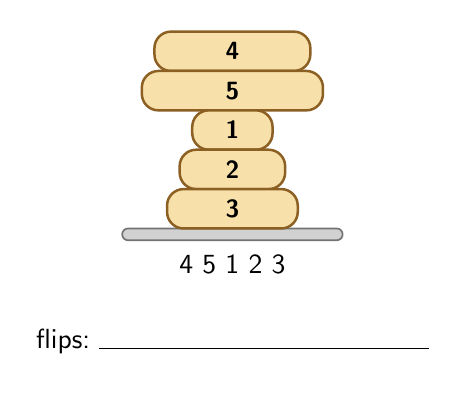
\begin{tikzpicture}
\useasboundingbox (-2.600,-1.880) rectangle (2.600,2.550);
\draw[platedraw, platefill, rounded corners=0.075cm] (-1.400,-0.150) rectangle (1.400,0);
\fill[cakefill] [rounded corners=0.210cm] (-0.990,2.000) rectangle (0.990,2.500);
\draw[cakedraw] [rounded corners=0.210cm] (-0.990,2.000) rectangle (0.990,2.500);
\node[font=\small\bfseries, inner sep=0pt] at (0.000,2.250) {4};
\fill[cakefill] [rounded corners=0.210cm] (-1.150,1.500) rectangle (1.150,2.000);
\draw[cakedraw] [rounded corners=0.210cm] (-1.150,1.500) rectangle (1.150,2.000);
\node[font=\small\bfseries, inner sep=0pt] at (0.000,1.750) {5};
\fill[cakefill] [rounded corners=0.210cm] (-0.510,1.000) rectangle (0.510,1.500);
\draw[cakedraw] [rounded corners=0.210cm] (-0.510,1.000) rectangle (0.510,1.500);
\node[font=\small\bfseries, inner sep=0pt] at (0.000,1.250) {1};
\fill[cakefill] [rounded corners=0.210cm] (-0.670,0.500) rectangle (0.670,1.000);
\draw[cakedraw] [rounded corners=0.210cm] (-0.670,0.500) rectangle (0.670,1.000);
\node[font=\small\bfseries, inner sep=0pt] at (0.000,0.750) {2};
\fill[cakefill] [rounded corners=0.210cm] (-0.830,0.000) rectangle (0.830,0.500);
\draw[cakedraw] [rounded corners=0.210cm] (-0.830,0.000) rectangle (0.830,0.500);
\node[font=\small\bfseries, inner sep=0pt] at (0.000,0.250) {3};
\node[anchor=north, font=\normalsize, inner sep=0pt] at (0.000,-0.330) {4\,\,5\,\,1\,\,2\,\,3};
\node[anchor=base west, font=\normalsize, inner sep=0pt] (fl) at (-2.500,-1.530) {flips:};
\draw[thin] ([xshift=3pt]fl.base east) -- (2.500,-1.530);
\end{tikzpicture}\hfill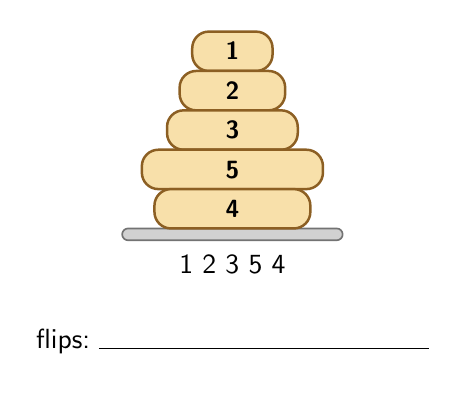
\begin{tikzpicture}
\useasboundingbox (-2.600,-1.880) rectangle (2.600,2.550);
\draw[platedraw, platefill, rounded corners=0.075cm] (-1.400,-0.150) rectangle (1.400,0);
\fill[cakefill] [rounded corners=0.210cm] (-0.510,2.000) rectangle (0.510,2.500);
\draw[cakedraw] [rounded corners=0.210cm] (-0.510,2.000) rectangle (0.510,2.500);
\node[font=\small\bfseries, inner sep=0pt] at (0.000,2.250) {1};
\fill[cakefill] [rounded corners=0.210cm] (-0.670,1.500) rectangle (0.670,2.000);
\draw[cakedraw] [rounded corners=0.210cm] (-0.670,1.500) rectangle (0.670,2.000);
\node[font=\small\bfseries, inner sep=0pt] at (0.000,1.750) {2};
\fill[cakefill] [rounded corners=0.210cm] (-0.830,1.000) rectangle (0.830,1.500);
\draw[cakedraw] [rounded corners=0.210cm] (-0.830,1.000) rectangle (0.830,1.500);
\node[font=\small\bfseries, inner sep=0pt] at (0.000,1.250) {3};
\fill[cakefill] [rounded corners=0.210cm] (-1.150,0.500) rectangle (1.150,1.000);
\draw[cakedraw] [rounded corners=0.210cm] (-1.150,0.500) rectangle (1.150,1.000);
\node[font=\small\bfseries, inner sep=0pt] at (0.000,0.750) {5};
\fill[cakefill] [rounded corners=0.210cm] (-0.990,0.000) rectangle (0.990,0.500);
\draw[cakedraw] [rounded corners=0.210cm] (-0.990,0.000) rectangle (0.990,0.500);
\node[font=\small\bfseries, inner sep=0pt] at (0.000,0.250) {4};
\node[anchor=north, font=\normalsize, inner sep=0pt] at (0.000,-0.330) {1\,\,2\,\,3\,\,5\,\,4};
\node[anchor=base west, font=\normalsize, inner sep=0pt] (fl) at (-2.500,-1.530) {flips:};
\draw[thin] ([xshift=3pt]fl.base east) -- (2.500,-1.530);
\end{tikzpicture}\hfill}

\newpage
\problem{2}Which stack of pancakes 1, 2 and 3 needs the most flips? Explain why it cannot be sorted in fewer.
\par\vspace{6.8cm}
\problem{3}Sort each stack of six with as few flips as you can.
\par\medskip
\noindent\makebox[\linewidth][s]{\hfill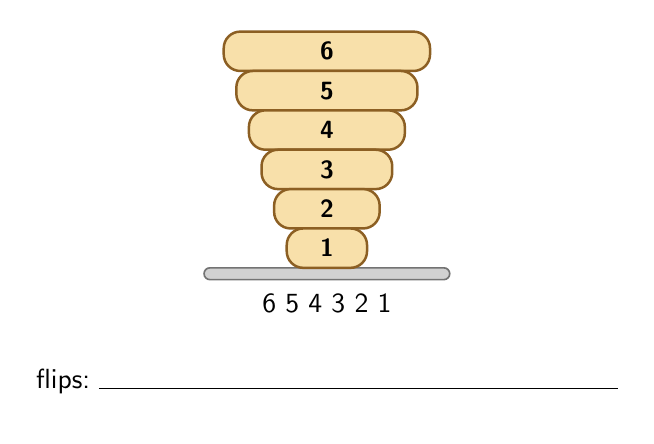
\begin{tikzpicture}
\useasboundingbox (-3.800,-1.880) rectangle (3.800,3.050);
\draw[platedraw, platefill, rounded corners=0.075cm] (-1.560,-0.150) rectangle (1.560,0);
\fill[cakefill] [rounded corners=0.210cm] (-1.310,2.500) rectangle (1.310,3.000);
\draw[cakedraw] [rounded corners=0.210cm] (-1.310,2.500) rectangle (1.310,3.000);
\node[font=\small\bfseries, inner sep=0pt] at (0.000,2.750) {6};
\fill[cakefill] [rounded corners=0.210cm] (-1.150,2.000) rectangle (1.150,2.500);
\draw[cakedraw] [rounded corners=0.210cm] (-1.150,2.000) rectangle (1.150,2.500);
\node[font=\small\bfseries, inner sep=0pt] at (0.000,2.250) {5};
\fill[cakefill] [rounded corners=0.210cm] (-0.990,1.500) rectangle (0.990,2.000);
\draw[cakedraw] [rounded corners=0.210cm] (-0.990,1.500) rectangle (0.990,2.000);
\node[font=\small\bfseries, inner sep=0pt] at (0.000,1.750) {4};
\fill[cakefill] [rounded corners=0.210cm] (-0.830,1.000) rectangle (0.830,1.500);
\draw[cakedraw] [rounded corners=0.210cm] (-0.830,1.000) rectangle (0.830,1.500);
\node[font=\small\bfseries, inner sep=0pt] at (0.000,1.250) {3};
\fill[cakefill] [rounded corners=0.210cm] (-0.670,0.500) rectangle (0.670,1.000);
\draw[cakedraw] [rounded corners=0.210cm] (-0.670,0.500) rectangle (0.670,1.000);
\node[font=\small\bfseries, inner sep=0pt] at (0.000,0.750) {2};
\fill[cakefill] [rounded corners=0.210cm] (-0.510,0.000) rectangle (0.510,0.500);
\draw[cakedraw] [rounded corners=0.210cm] (-0.510,0.000) rectangle (0.510,0.500);
\node[font=\small\bfseries, inner sep=0pt] at (0.000,0.250) {1};
\node[anchor=north, font=\normalsize, inner sep=0pt] at (0.000,-0.330) {6\,\,5\,\,4\,\,3\,\,2\,\,1};
\node[anchor=base west, font=\normalsize, inner sep=0pt] (fl) at (-3.700,-1.530) {flips:};
\draw[thin] ([xshift=3pt]fl.base east) -- (3.700,-1.530);
\end{tikzpicture}\hfill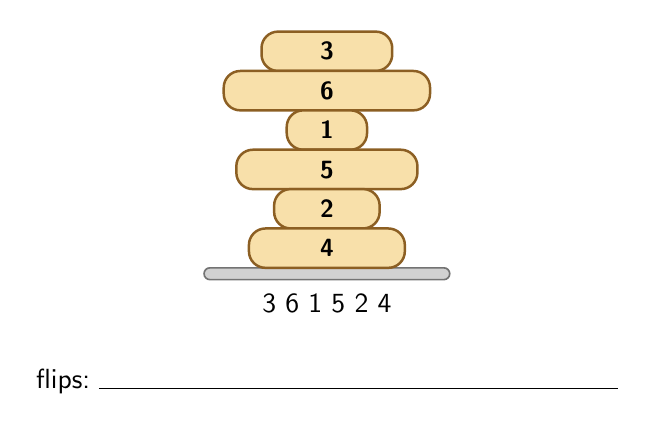
\begin{tikzpicture}
\useasboundingbox (-3.800,-1.880) rectangle (3.800,3.050);
\draw[platedraw, platefill, rounded corners=0.075cm] (-1.560,-0.150) rectangle (1.560,0);
\fill[cakefill] [rounded corners=0.210cm] (-0.830,2.500) rectangle (0.830,3.000);
\draw[cakedraw] [rounded corners=0.210cm] (-0.830,2.500) rectangle (0.830,3.000);
\node[font=\small\bfseries, inner sep=0pt] at (0.000,2.750) {3};
\fill[cakefill] [rounded corners=0.210cm] (-1.310,2.000) rectangle (1.310,2.500);
\draw[cakedraw] [rounded corners=0.210cm] (-1.310,2.000) rectangle (1.310,2.500);
\node[font=\small\bfseries, inner sep=0pt] at (0.000,2.250) {6};
\fill[cakefill] [rounded corners=0.210cm] (-0.510,1.500) rectangle (0.510,2.000);
\draw[cakedraw] [rounded corners=0.210cm] (-0.510,1.500) rectangle (0.510,2.000);
\node[font=\small\bfseries, inner sep=0pt] at (0.000,1.750) {1};
\fill[cakefill] [rounded corners=0.210cm] (-1.150,1.000) rectangle (1.150,1.500);
\draw[cakedraw] [rounded corners=0.210cm] (-1.150,1.000) rectangle (1.150,1.500);
\node[font=\small\bfseries, inner sep=0pt] at (0.000,1.250) {5};
\fill[cakefill] [rounded corners=0.210cm] (-0.670,0.500) rectangle (0.670,1.000);
\draw[cakedraw] [rounded corners=0.210cm] (-0.670,0.500) rectangle (0.670,1.000);
\node[font=\small\bfseries, inner sep=0pt] at (0.000,0.750) {2};
\fill[cakefill] [rounded corners=0.210cm] (-0.990,0.000) rectangle (0.990,0.500);
\draw[cakedraw] [rounded corners=0.210cm] (-0.990,0.000) rectangle (0.990,0.500);
\node[font=\small\bfseries, inner sep=0pt] at (0.000,0.250) {4};
\node[anchor=north, font=\normalsize, inner sep=0pt] at (0.000,-0.330) {3\,\,6\,\,1\,\,5\,\,2\,\,4};
\node[anchor=base west, font=\normalsize, inner sep=0pt] (fl) at (-3.700,-1.530) {flips:};
\draw[thin] ([xshift=3pt]fl.base east) -- (3.700,-1.530);
\end{tikzpicture}\hfill}

\par\vspace{0.7cm}
\noindent\makebox[\linewidth][s]{\hfill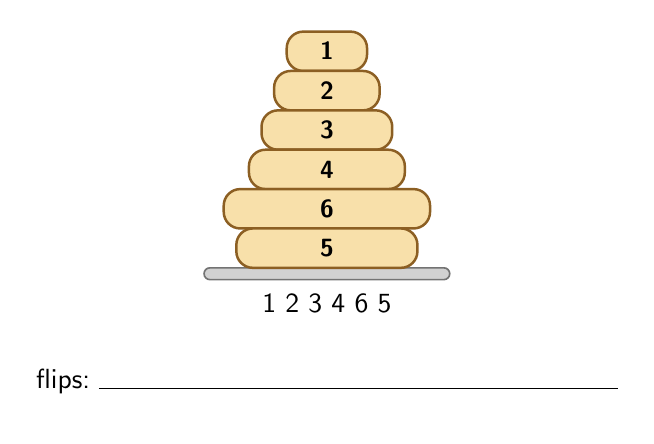
\begin{tikzpicture}
\useasboundingbox (-3.800,-1.880) rectangle (3.800,3.050);
\draw[platedraw, platefill, rounded corners=0.075cm] (-1.560,-0.150) rectangle (1.560,0);
\fill[cakefill] [rounded corners=0.210cm] (-0.510,2.500) rectangle (0.510,3.000);
\draw[cakedraw] [rounded corners=0.210cm] (-0.510,2.500) rectangle (0.510,3.000);
\node[font=\small\bfseries, inner sep=0pt] at (0.000,2.750) {1};
\fill[cakefill] [rounded corners=0.210cm] (-0.670,2.000) rectangle (0.670,2.500);
\draw[cakedraw] [rounded corners=0.210cm] (-0.670,2.000) rectangle (0.670,2.500);
\node[font=\small\bfseries, inner sep=0pt] at (0.000,2.250) {2};
\fill[cakefill] [rounded corners=0.210cm] (-0.830,1.500) rectangle (0.830,2.000);
\draw[cakedraw] [rounded corners=0.210cm] (-0.830,1.500) rectangle (0.830,2.000);
\node[font=\small\bfseries, inner sep=0pt] at (0.000,1.750) {3};
\fill[cakefill] [rounded corners=0.210cm] (-0.990,1.000) rectangle (0.990,1.500);
\draw[cakedraw] [rounded corners=0.210cm] (-0.990,1.000) rectangle (0.990,1.500);
\node[font=\small\bfseries, inner sep=0pt] at (0.000,1.250) {4};
\fill[cakefill] [rounded corners=0.210cm] (-1.310,0.500) rectangle (1.310,1.000);
\draw[cakedraw] [rounded corners=0.210cm] (-1.310,0.500) rectangle (1.310,1.000);
\node[font=\small\bfseries, inner sep=0pt] at (0.000,0.750) {6};
\fill[cakefill] [rounded corners=0.210cm] (-1.150,0.000) rectangle (1.150,0.500);
\draw[cakedraw] [rounded corners=0.210cm] (-1.150,0.000) rectangle (1.150,0.500);
\node[font=\small\bfseries, inner sep=0pt] at (0.000,0.250) {5};
\node[anchor=north, font=\normalsize, inner sep=0pt] at (0.000,-0.330) {1\,\,2\,\,3\,\,4\,\,6\,\,5};
\node[anchor=base west, font=\normalsize, inner sep=0pt] (fl) at (-3.700,-1.530) {flips:};
\draw[thin] ([xshift=3pt]fl.base east) -- (3.700,-1.530);
\end{tikzpicture}\hfill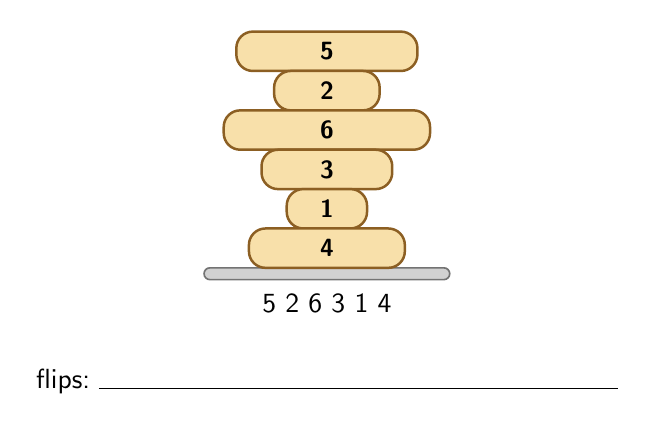
\begin{tikzpicture}
\useasboundingbox (-3.800,-1.880) rectangle (3.800,3.050);
\draw[platedraw, platefill, rounded corners=0.075cm] (-1.560,-0.150) rectangle (1.560,0);
\fill[cakefill] [rounded corners=0.210cm] (-1.150,2.500) rectangle (1.150,3.000);
\draw[cakedraw] [rounded corners=0.210cm] (-1.150,2.500) rectangle (1.150,3.000);
\node[font=\small\bfseries, inner sep=0pt] at (0.000,2.750) {5};
\fill[cakefill] [rounded corners=0.210cm] (-0.670,2.000) rectangle (0.670,2.500);
\draw[cakedraw] [rounded corners=0.210cm] (-0.670,2.000) rectangle (0.670,2.500);
\node[font=\small\bfseries, inner sep=0pt] at (0.000,2.250) {2};
\fill[cakefill] [rounded corners=0.210cm] (-1.310,1.500) rectangle (1.310,2.000);
\draw[cakedraw] [rounded corners=0.210cm] (-1.310,1.500) rectangle (1.310,2.000);
\node[font=\small\bfseries, inner sep=0pt] at (0.000,1.750) {6};
\fill[cakefill] [rounded corners=0.210cm] (-0.830,1.000) rectangle (0.830,1.500);
\draw[cakedraw] [rounded corners=0.210cm] (-0.830,1.000) rectangle (0.830,1.500);
\node[font=\small\bfseries, inner sep=0pt] at (0.000,1.250) {3};
\fill[cakefill] [rounded corners=0.210cm] (-0.510,0.500) rectangle (0.510,1.000);
\draw[cakedraw] [rounded corners=0.210cm] (-0.510,0.500) rectangle (0.510,1.000);
\node[font=\small\bfseries, inner sep=0pt] at (0.000,0.750) {1};
\fill[cakefill] [rounded corners=0.210cm] (-0.990,0.000) rectangle (0.990,0.500);
\draw[cakedraw] [rounded corners=0.210cm] (-0.990,0.000) rectangle (0.990,0.500);
\node[font=\small\bfseries, inner sep=0pt] at (0.000,0.250) {4};
\node[anchor=north, font=\normalsize, inner sep=0pt] at (0.000,-0.330) {5\,\,2\,\,6\,\,3\,\,1\,\,4};
\node[anchor=base west, font=\normalsize, inner sep=0pt] (fl) at (-3.700,-1.530) {flips:};
\draw[thin] ([xshift=3pt]fl.base east) -- (3.700,-1.530);
\end{tikzpicture}\hfill}

\newpage
\problem{4}Find a way to sort any stack of six pancakes, however mixed up it is. What is the most flips your way can need? What about a stack of ten pancakes?
\newpage
\problem{5}Find all the stacks of pancakes 1, 2, 3 and 4 that cannot be sorted in three flips or fewer.
\newpage
\problem{6}Now each pancake has a dark side, which must end facing down. Sort each stack with as few flips as you can.
\par\smallskip\begin{center}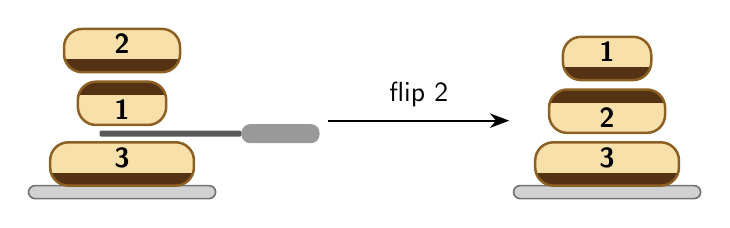
\begin{tikzpicture}
\draw[platedraw, platefill, rounded corners=0.083cm] (-1.188,-0.165) rectangle (1.188,0);
\fill[cakefill] [rounded corners=0.231cm] (-0.737,1.440) rectangle (0.737,1.990);
\begin{scope}
\clip [rounded corners=0.231cm] (-0.737,1.440) rectangle (0.737,1.990);
\fill[burnt] (-0.737,1.440) rectangle (0.737,1.605);
\end{scope}
\draw[cakedraw] [rounded corners=0.231cm] (-0.737,1.440) rectangle (0.737,1.990);
\node[font=\normalsize\bfseries, inner sep=0pt] at (0.000,1.797) {2};
\fill[cakefill] [rounded corners=0.231cm] (-0.561,0.770) rectangle (0.561,1.320);
\begin{scope}
\clip [rounded corners=0.231cm] (-0.561,0.770) rectangle (0.561,1.320);
\fill[burnt] (-0.561,1.155) rectangle (0.561,1.320);
\end{scope}
\draw[cakedraw] [rounded corners=0.231cm] (-0.561,0.770) rectangle (0.561,1.320);
\node[font=\normalsize\bfseries, inner sep=0pt] at (0.000,0.963) {1};
\fill[cakefill] [rounded corners=0.231cm] (-0.913,0.000) rectangle (0.913,0.550);
\begin{scope}
\clip [rounded corners=0.231cm] (-0.913,0.000) rectangle (0.913,0.550);
\fill[burnt] (-0.913,0.000) rectangle (0.913,0.165);
\end{scope}
\draw[cakedraw] [rounded corners=0.231cm] (-0.913,0.000) rectangle (0.913,0.550);
\node[font=\normalsize\bfseries, inner sep=0pt] at (0.000,0.358) {3};
\fill[spatula, rounded corners=0.5pt] (-0.286,0.622) rectangle (1.518,0.699);
\fill[handle, rounded corners=0.109cm] (1.518,0.539) rectangle (2.508,0.781);
\draw[-{Stealth[length=7pt]}, thick] (2.618,0.825) -- (4.917,0.825);
\node[above, font=\normalsize] at (3.768,0.875) {flip 2};
\draw[platedraw, platefill, rounded corners=0.083cm] (4.972,-0.165) rectangle (7.348,0);
\fill[cakefill] [rounded corners=0.231cm] (5.599,1.340) rectangle (6.721,1.890);
\begin{scope}
\clip [rounded corners=0.231cm] (5.599,1.340) rectangle (6.721,1.890);
\fill[burnt] (5.599,1.340) rectangle (6.721,1.505);
\end{scope}
\draw[cakedraw] [rounded corners=0.231cm] (5.599,1.340) rectangle (6.721,1.890);
\node[font=\normalsize\bfseries, inner sep=0pt] at (6.160,1.698) {1};
\fill[cakefill] [rounded corners=0.231cm] (5.423,0.670) rectangle (6.897,1.220);
\begin{scope}
\clip [rounded corners=0.231cm] (5.423,0.670) rectangle (6.897,1.220);
\fill[burnt] (5.423,1.055) rectangle (6.897,1.220);
\end{scope}
\draw[cakedraw] [rounded corners=0.231cm] (5.423,0.670) rectangle (6.897,1.220);
\node[font=\normalsize\bfseries, inner sep=0pt] at (6.160,0.863) {2};
\fill[cakefill] [rounded corners=0.231cm] (5.247,0.000) rectangle (7.073,0.550);
\begin{scope}
\clip [rounded corners=0.231cm] (5.247,0.000) rectangle (7.073,0.550);
\fill[burnt] (5.247,0.000) rectangle (7.073,0.165);
\end{scope}
\draw[cakedraw] [rounded corners=0.231cm] (5.247,0.000) rectangle (7.073,0.550);
\node[font=\normalsize\bfseries, inner sep=0pt] at (6.160,0.358) {3};
\end{tikzpicture}\end{center}
\par\medskip
\noindent\makebox[\linewidth][s]{\hfill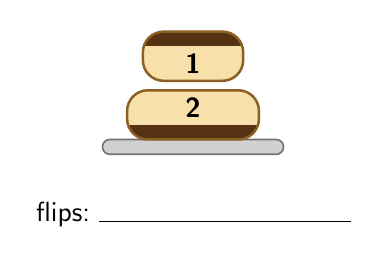
\begin{tikzpicture}
\useasboundingbox (-2.100,-1.388) rectangle (2.100,1.420);
\draw[platedraw, platefill, rounded corners=0.094cm] (-1.150,-0.188) rectangle (1.150,0);
\fill[cakefill] [rounded corners=0.263cm] (-0.637,0.745) rectangle (0.637,1.370);
\begin{scope}
\clip [rounded corners=0.263cm] (-0.637,0.745) rectangle (0.637,1.370);
\fill[burnt] (-0.637,1.183) rectangle (0.637,1.370);
\end{scope}
\draw[cakedraw] [rounded corners=0.263cm] (-0.637,0.745) rectangle (0.637,1.370);
\node[font=\normalsize\bfseries, inner sep=0pt] at (0.000,0.964) {1};
\fill[cakefill] [rounded corners=0.263cm] (-0.837,0.000) rectangle (0.837,0.625);
\begin{scope}
\clip [rounded corners=0.263cm] (-0.837,0.000) rectangle (0.837,0.625);
\fill[burnt] (-0.837,0.000) rectangle (0.837,0.188);
\end{scope}
\draw[cakedraw] [rounded corners=0.263cm] (-0.837,0.000) rectangle (0.837,0.625);
\node[font=\normalsize\bfseries, inner sep=0pt] at (0.000,0.406) {2};
\node[anchor=base west, font=\normalsize, inner sep=0pt] (fl) at (-2.000,-1.038) {flips:};
\draw[thin] ([xshift=3pt]fl.base east) -- (2.000,-1.038);
\end{tikzpicture}\hfill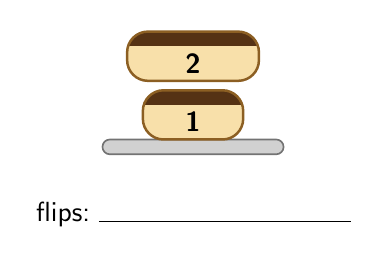
\begin{tikzpicture}
\useasboundingbox (-2.100,-1.388) rectangle (2.100,1.420);
\draw[platedraw, platefill, rounded corners=0.094cm] (-1.150,-0.188) rectangle (1.150,0);
\fill[cakefill] [rounded corners=0.263cm] (-0.837,0.745) rectangle (0.837,1.370);
\begin{scope}
\clip [rounded corners=0.263cm] (-0.837,0.745) rectangle (0.837,1.370);
\fill[burnt] (-0.837,1.183) rectangle (0.837,1.370);
\end{scope}
\draw[cakedraw] [rounded corners=0.263cm] (-0.837,0.745) rectangle (0.837,1.370);
\node[font=\normalsize\bfseries, inner sep=0pt] at (0.000,0.964) {2};
\fill[cakefill] [rounded corners=0.263cm] (-0.637,0.000) rectangle (0.637,0.625);
\begin{scope}
\clip [rounded corners=0.263cm] (-0.637,0.000) rectangle (0.637,0.625);
\fill[burnt] (-0.637,0.438) rectangle (0.637,0.625);
\end{scope}
\draw[cakedraw] [rounded corners=0.263cm] (-0.637,0.000) rectangle (0.637,0.625);
\node[font=\normalsize\bfseries, inner sep=0pt] at (0.000,0.219) {1};
\node[anchor=base west, font=\normalsize, inner sep=0pt] (fl) at (-2.000,-1.038) {flips:};
\draw[thin] ([xshift=3pt]fl.base east) -- (2.000,-1.038);
\end{tikzpicture}\hfill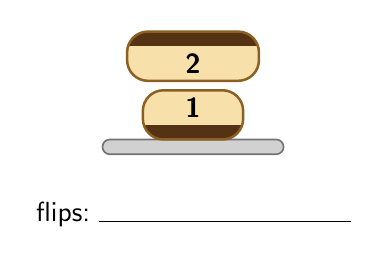
\begin{tikzpicture}
\useasboundingbox (-2.100,-1.388) rectangle (2.100,1.420);
\draw[platedraw, platefill, rounded corners=0.094cm] (-1.150,-0.188) rectangle (1.150,0);
\fill[cakefill] [rounded corners=0.263cm] (-0.837,0.745) rectangle (0.837,1.370);
\begin{scope}
\clip [rounded corners=0.263cm] (-0.837,0.745) rectangle (0.837,1.370);
\fill[burnt] (-0.837,1.183) rectangle (0.837,1.370);
\end{scope}
\draw[cakedraw] [rounded corners=0.263cm] (-0.837,0.745) rectangle (0.837,1.370);
\node[font=\normalsize\bfseries, inner sep=0pt] at (0.000,0.964) {2};
\fill[cakefill] [rounded corners=0.263cm] (-0.637,0.000) rectangle (0.637,0.625);
\begin{scope}
\clip [rounded corners=0.263cm] (-0.637,0.000) rectangle (0.637,0.625);
\fill[burnt] (-0.637,0.000) rectangle (0.637,0.188);
\end{scope}
\draw[cakedraw] [rounded corners=0.263cm] (-0.637,0.000) rectangle (0.637,0.625);
\node[font=\normalsize\bfseries, inner sep=0pt] at (0.000,0.406) {1};
\node[anchor=base west, font=\normalsize, inner sep=0pt] (fl) at (-2.000,-1.038) {flips:};
\draw[thin] ([xshift=3pt]fl.base east) -- (2.000,-1.038);
\end{tikzpicture}\hfill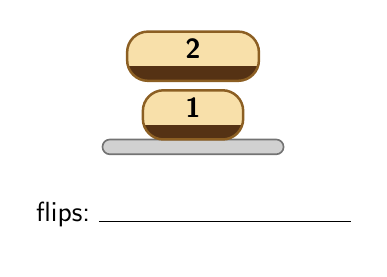
\begin{tikzpicture}
\useasboundingbox (-2.100,-1.388) rectangle (2.100,1.420);
\draw[platedraw, platefill, rounded corners=0.094cm] (-1.150,-0.188) rectangle (1.150,0);
\fill[cakefill] [rounded corners=0.263cm] (-0.837,0.745) rectangle (0.837,1.370);
\begin{scope}
\clip [rounded corners=0.263cm] (-0.837,0.745) rectangle (0.837,1.370);
\fill[burnt] (-0.837,0.745) rectangle (0.837,0.932);
\end{scope}
\draw[cakedraw] [rounded corners=0.263cm] (-0.837,0.745) rectangle (0.837,1.370);
\node[font=\normalsize\bfseries, inner sep=0pt] at (0.000,1.151) {2};
\fill[cakefill] [rounded corners=0.263cm] (-0.637,0.000) rectangle (0.637,0.625);
\begin{scope}
\clip [rounded corners=0.263cm] (-0.637,0.000) rectangle (0.637,0.625);
\fill[burnt] (-0.637,0.000) rectangle (0.637,0.188);
\end{scope}
\draw[cakedraw] [rounded corners=0.263cm] (-0.637,0.000) rectangle (0.637,0.625);
\node[font=\normalsize\bfseries, inner sep=0pt] at (0.000,0.406) {1};
\node[anchor=base west, font=\normalsize, inner sep=0pt] (fl) at (-2.000,-1.038) {flips:};
\draw[thin] ([xshift=3pt]fl.base east) -- (2.000,-1.038);
\end{tikzpicture}\hfill}

\par\vspace{1.2cm}
\problem{7}Find the stack of pancakes 1 and 2 that needs the most flips. Draw it with its dark sides.
\par\bigskip
\noindent\makebox[\linewidth][s]{\hfill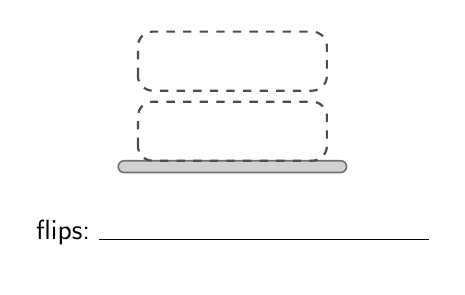
\begin{tikzpicture}
\useasboundingbox (-2.600,-1.350) rectangle (2.600,1.690);
\draw[platedraw, platefill, rounded corners=0.075cm] (-1.450,-0.150) rectangle (1.450,0);
\draw[slot, rounded corners=0.188cm] (-1.200,0.890) rectangle (1.200,1.640);
\draw[slot, rounded corners=0.188cm] (-1.200,0.000) rectangle (1.200,0.750);
\node[anchor=base west, font=\normalsize, inner sep=0pt] (fl) at (-2.500,-1.000) {flips:};
\draw[thin] ([xshift=3pt]fl.base east) -- (2.500,-1.000);
\end{tikzpicture}\hfill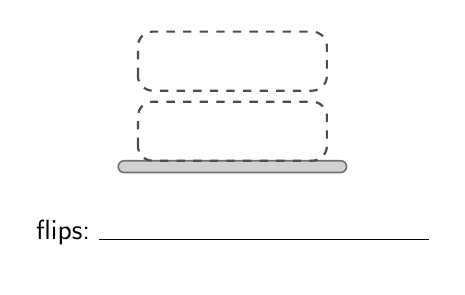
\begin{tikzpicture}
\useasboundingbox (-2.600,-1.350) rectangle (2.600,1.690);
\draw[platedraw, platefill, rounded corners=0.075cm] (-1.450,-0.150) rectangle (1.450,0);
\draw[slot, rounded corners=0.188cm] (-1.200,0.890) rectangle (1.200,1.640);
\draw[slot, rounded corners=0.188cm] (-1.200,0.000) rectangle (1.200,0.750);
\node[anchor=base west, font=\normalsize, inner sep=0pt] (fl) at (-2.500,-1.000) {flips:};
\draw[thin] ([xshift=3pt]fl.base east) -- (2.500,-1.000);
\end{tikzpicture}\hfill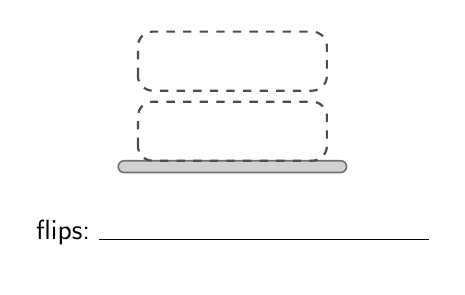
\begin{tikzpicture}
\useasboundingbox (-2.600,-1.350) rectangle (2.600,1.690);
\draw[platedraw, platefill, rounded corners=0.075cm] (-1.450,-0.150) rectangle (1.450,0);
\draw[slot, rounded corners=0.188cm] (-1.200,0.890) rectangle (1.200,1.640);
\draw[slot, rounded corners=0.188cm] (-1.200,0.000) rectangle (1.200,0.750);
\node[anchor=base west, font=\normalsize, inner sep=0pt] (fl) at (-2.500,-1.000) {flips:};
\draw[thin] ([xshift=3pt]fl.base east) -- (2.500,-1.000);
\end{tikzpicture}\hfill}

\newpage
\problem{8}Sort each stack of three so that every dark side ends facing down, with as few flips as you can.
\par\medskip
\noindent\makebox[\linewidth][s]{\hfill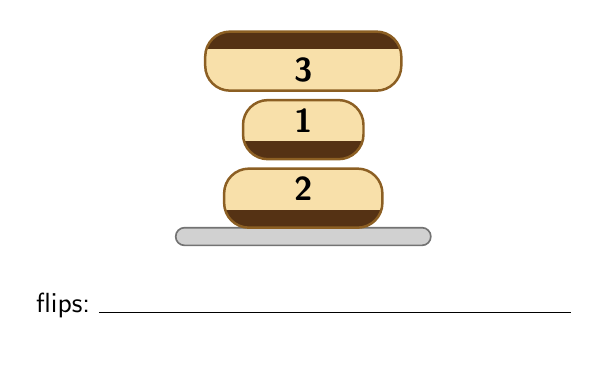
\begin{tikzpicture}
\useasboundingbox (-3.500,-1.425) rectangle (3.500,2.540);
\draw[platedraw, platefill, rounded corners=0.112cm] (-1.620,-0.225) rectangle (1.620,0);
\fill[cakefill] [rounded corners=0.315cm] (-1.245,1.740) rectangle (1.245,2.490);
\begin{scope}
\clip [rounded corners=0.315cm] (-1.245,1.740) rectangle (1.245,2.490);
\fill[burnt] (-1.245,2.265) rectangle (1.245,2.490);
\end{scope}
\draw[cakedraw] [rounded corners=0.315cm] (-1.245,1.740) rectangle (1.245,2.490);
\node[font=\large\bfseries, inner sep=0pt] at (0.000,2.003) {3};
\fill[cakefill] [rounded corners=0.315cm] (-0.765,0.870) rectangle (0.765,1.620);
\begin{scope}
\clip [rounded corners=0.315cm] (-0.765,0.870) rectangle (0.765,1.620);
\fill[burnt] (-0.765,0.870) rectangle (0.765,1.095);
\end{scope}
\draw[cakedraw] [rounded corners=0.315cm] (-0.765,0.870) rectangle (0.765,1.620);
\node[font=\large\bfseries, inner sep=0pt] at (0.000,1.357) {1};
\fill[cakefill] [rounded corners=0.315cm] (-1.005,0.000) rectangle (1.005,0.750);
\begin{scope}
\clip [rounded corners=0.315cm] (-1.005,0.000) rectangle (1.005,0.750);
\fill[burnt] (-1.005,0.000) rectangle (1.005,0.225);
\end{scope}
\draw[cakedraw] [rounded corners=0.315cm] (-1.005,0.000) rectangle (1.005,0.750);
\node[font=\large\bfseries, inner sep=0pt] at (0.000,0.487) {2};
\node[anchor=base west, font=\normalsize, inner sep=0pt] (fl) at (-3.400,-1.075) {flips:};
\draw[thin] ([xshift=3pt]fl.base east) -- (3.400,-1.075);
\end{tikzpicture}\hfill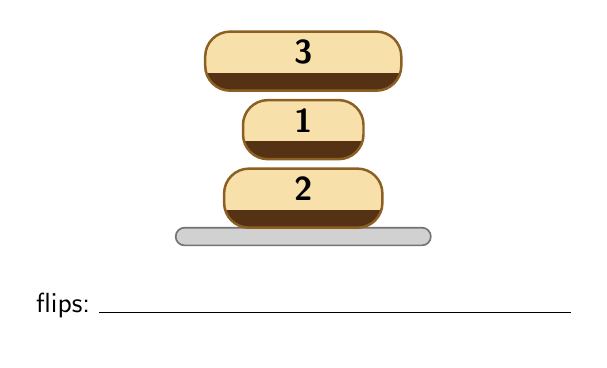
\begin{tikzpicture}
\useasboundingbox (-3.500,-1.425) rectangle (3.500,2.540);
\draw[platedraw, platefill, rounded corners=0.112cm] (-1.620,-0.225) rectangle (1.620,0);
\fill[cakefill] [rounded corners=0.315cm] (-1.245,1.740) rectangle (1.245,2.490);
\begin{scope}
\clip [rounded corners=0.315cm] (-1.245,1.740) rectangle (1.245,2.490);
\fill[burnt] (-1.245,1.740) rectangle (1.245,1.965);
\end{scope}
\draw[cakedraw] [rounded corners=0.315cm] (-1.245,1.740) rectangle (1.245,2.490);
\node[font=\large\bfseries, inner sep=0pt] at (0.000,2.228) {3};
\fill[cakefill] [rounded corners=0.315cm] (-0.765,0.870) rectangle (0.765,1.620);
\begin{scope}
\clip [rounded corners=0.315cm] (-0.765,0.870) rectangle (0.765,1.620);
\fill[burnt] (-0.765,0.870) rectangle (0.765,1.095);
\end{scope}
\draw[cakedraw] [rounded corners=0.315cm] (-0.765,0.870) rectangle (0.765,1.620);
\node[font=\large\bfseries, inner sep=0pt] at (0.000,1.357) {1};
\fill[cakefill] [rounded corners=0.315cm] (-1.005,0.000) rectangle (1.005,0.750);
\begin{scope}
\clip [rounded corners=0.315cm] (-1.005,0.000) rectangle (1.005,0.750);
\fill[burnt] (-1.005,0.000) rectangle (1.005,0.225);
\end{scope}
\draw[cakedraw] [rounded corners=0.315cm] (-1.005,0.000) rectangle (1.005,0.750);
\node[font=\large\bfseries, inner sep=0pt] at (0.000,0.487) {2};
\node[anchor=base west, font=\normalsize, inner sep=0pt] (fl) at (-3.400,-1.075) {flips:};
\draw[thin] ([xshift=3pt]fl.base east) -- (3.400,-1.075);
\end{tikzpicture}\hfill}

\par\vspace{1.2cm}
\noindent\makebox[\linewidth][s]{\hfill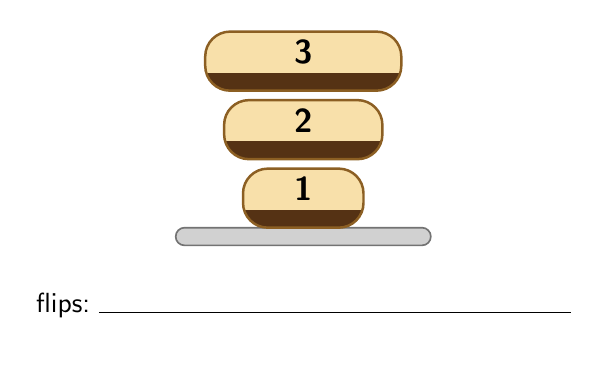
\begin{tikzpicture}
\useasboundingbox (-3.500,-1.425) rectangle (3.500,2.540);
\draw[platedraw, platefill, rounded corners=0.112cm] (-1.620,-0.225) rectangle (1.620,0);
\fill[cakefill] [rounded corners=0.315cm] (-1.245,1.740) rectangle (1.245,2.490);
\begin{scope}
\clip [rounded corners=0.315cm] (-1.245,1.740) rectangle (1.245,2.490);
\fill[burnt] (-1.245,1.740) rectangle (1.245,1.965);
\end{scope}
\draw[cakedraw] [rounded corners=0.315cm] (-1.245,1.740) rectangle (1.245,2.490);
\node[font=\large\bfseries, inner sep=0pt] at (0.000,2.228) {3};
\fill[cakefill] [rounded corners=0.315cm] (-1.005,0.870) rectangle (1.005,1.620);
\begin{scope}
\clip [rounded corners=0.315cm] (-1.005,0.870) rectangle (1.005,1.620);
\fill[burnt] (-1.005,0.870) rectangle (1.005,1.095);
\end{scope}
\draw[cakedraw] [rounded corners=0.315cm] (-1.005,0.870) rectangle (1.005,1.620);
\node[font=\large\bfseries, inner sep=0pt] at (0.000,1.357) {2};
\fill[cakefill] [rounded corners=0.315cm] (-0.765,0.000) rectangle (0.765,0.750);
\begin{scope}
\clip [rounded corners=0.315cm] (-0.765,0.000) rectangle (0.765,0.750);
\fill[burnt] (-0.765,0.000) rectangle (0.765,0.225);
\end{scope}
\draw[cakedraw] [rounded corners=0.315cm] (-0.765,0.000) rectangle (0.765,0.750);
\node[font=\large\bfseries, inner sep=0pt] at (0.000,0.487) {1};
\node[anchor=base west, font=\normalsize, inner sep=0pt] (fl) at (-3.400,-1.075) {flips:};
\draw[thin] ([xshift=3pt]fl.base east) -- (3.400,-1.075);
\end{tikzpicture}\hfill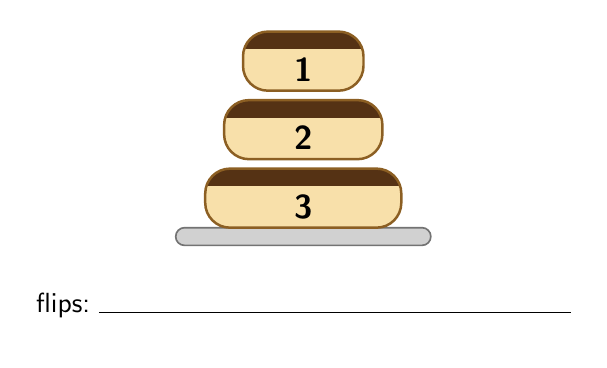
\begin{tikzpicture}
\useasboundingbox (-3.500,-1.425) rectangle (3.500,2.540);
\draw[platedraw, platefill, rounded corners=0.112cm] (-1.620,-0.225) rectangle (1.620,0);
\fill[cakefill] [rounded corners=0.315cm] (-0.765,1.740) rectangle (0.765,2.490);
\begin{scope}
\clip [rounded corners=0.315cm] (-0.765,1.740) rectangle (0.765,2.490);
\fill[burnt] (-0.765,2.265) rectangle (0.765,2.490);
\end{scope}
\draw[cakedraw] [rounded corners=0.315cm] (-0.765,1.740) rectangle (0.765,2.490);
\node[font=\large\bfseries, inner sep=0pt] at (0.000,2.003) {1};
\fill[cakefill] [rounded corners=0.315cm] (-1.005,0.870) rectangle (1.005,1.620);
\begin{scope}
\clip [rounded corners=0.315cm] (-1.005,0.870) rectangle (1.005,1.620);
\fill[burnt] (-1.005,1.395) rectangle (1.005,1.620);
\end{scope}
\draw[cakedraw] [rounded corners=0.315cm] (-1.005,0.870) rectangle (1.005,1.620);
\node[font=\large\bfseries, inner sep=0pt] at (0.000,1.133) {2};
\fill[cakefill] [rounded corners=0.315cm] (-1.245,0.000) rectangle (1.245,0.750);
\begin{scope}
\clip [rounded corners=0.315cm] (-1.245,0.000) rectangle (1.245,0.750);
\fill[burnt] (-1.245,0.525) rectangle (1.245,0.750);
\end{scope}
\draw[cakedraw] [rounded corners=0.315cm] (-1.245,0.000) rectangle (1.245,0.750);
\node[font=\large\bfseries, inner sep=0pt] at (0.000,0.263) {3};
\node[anchor=base west, font=\normalsize, inner sep=0pt] (fl) at (-3.400,-1.075) {flips:};
\draw[thin] ([xshift=3pt]fl.base east) -- (3.400,-1.075);
\end{tikzpicture}\hfill}

\end{document}
